\documentclass[border=2mm]{standalone}

\usepackage{amsmath}
\usepackage{pgfplots}
\pgfplotsset{compat=1.18}
\usetikzlibrary{arrows.meta, calc, positioning, decorations.pathreplacing, calligraphy}

\usepackage{xcolor}
\definecolor{den-1}{HTML}{111111}   % Đen #111111
\definecolor{den-2}{HTML}{222222}   % Đen #222222
\definecolor{den-3}{HTML}{333333}   % Đen #333333
\definecolor{den-4}{HTML}{444444}   % Đen #444444
\definecolor{den-5}{HTML}{555555}   % Đen #555555
\definecolor{den-6}{HTML}{666666}   % Đen #666666

\tikzset{
  >=Stealth,
  originlabel/.style={
    font=\small\sf,
    anchor=north east, 
    yshift=-0.1ex,     
    xshift=-0.1ex      
  }
}

\begin{document}

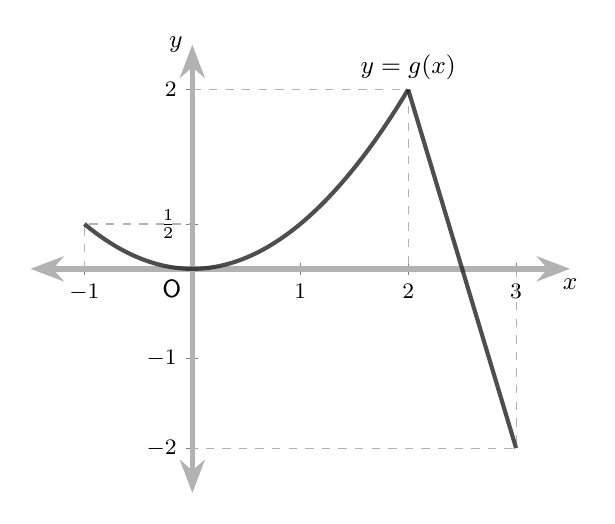
\begin{tikzpicture}

\begin{axis}[
    font=\small\sf,
    axis lines=middle,
    axis line style={<->, line width=2pt, color=den-6!50},
    xlabel=$x$, ylabel=$y$,
    xlabel style={below, font=\small\sf},
    ylabel style={left, font=\small\sf},
    xmin=-1.5, xmax=3.5,
    ymin=-2.5, ymax=2.5,
    xtick={-1, 1, 2, 3},
    ytick={-2, -1, .5, 2},
    xticklabels={$-1$, $1$, $2$, $3$},
    yticklabels={$-2$, $-1$, $\frac{1}{2}$, $2$},
    tick label style={font=\footnotesize\sf},
    clip=false,
]

\node[originlabel] at (axis cs:0,0) {O};

\draw [dashed, color=den-6!50] (-1,0) -- (-1,.5) -- (0,.5);

\draw [dashed, color=den-6!50] (0,2) -- (2,2) -- (2,0);

\draw [dashed, color=den-6!50] (3,0) -- (3,-2) -- (0,-2);

\addplot[domain=-1:2, samples=100, line width=1.5pt, color=den-2, opacity=.8] {.5*x^2};

\addplot[domain=2:3, samples=100, line width=1.5pt, color=den-2, opacity=.8] {-4*x+10};

\node at (2,2) [anchor=south] {$y=g(x)$};

\end{axis}

\end{tikzpicture}

\end{document}
